\documentclass[handout]{beamer}
\usepackage{tikz}
\usetikzlibrary{shapes.geometric, arrows.meta, positioning}
\tikzstyle{startstop} = [
  rectangle, rounded corners, minimum width=3cm, 
  minimum height=1cm,  text width=3cm, text centered,
  align=center, draw=black, fill=white]
\tikzstyle{arrow} = [thick, ->, >=stealth]

\usepackage{graphicx}
\usepackage{xcolor}
\usepackage{multirow}
\setbeamertemplate{blocks}[rounded][shadow=true] % estilo de bloque
\setbeamercolor{block body}{bg=white, fg=black}  % fondo y texto
\setbeamercolor{block title}{bg=blue!20, fg=black} % título
%Information to be included in the title page:
\title{Aprendizaje por Refuerzo \newline
Métodos Computacionales}
\author{Daniela Pucci de Farias}
\institute{Universidad Torcuato Di Tella}
\date{June 2025}

\begin{document}

\frame{\titlepage}

\begin{frame}{Clase 4}
\begin{itemize}
\item Computación en MDPs
\begin{itemize}
\item Iteración de valor
\item Iteración de política
\end{itemize}
\item<2-> Desafíos en MDPs
\begin{itemize}
\item Incertidumbre y/o complejidad del ambiente
\item “Curse of dimensionality” (la maldición de la dimensionalidad)
\end{itemize}
\item<3-> Métodos de Aprendizaje por Refuerzo
\begin{itemize}
\item Simulación Monte Carlo 
\item TD-Learning
\item Q-Learning
\end{itemize}
\end{itemize}
\end{frame}

\begin{frame}{Revisión: MDPs}
\begin{itemize}
\item MDP: tupla $(S,A, P, r)$
\item<2-> Ecuación de Bellman y función valor:
$$
V^*(x) =  \max\limits_{a \in A} 
\left\{r_a(x)+\alpha \sum_y P_a(x,y) V^*(y)\right\}
$$
\item<3-> Función de política óptima:
$$
u^*(x) =  \arg\max\limits_{a \in A} \left\{r_a(x)+\alpha \sum_y P_a(x,y) V^*(y)\right\}
$$
\item<4-> Algoritmos para resolver la ecuación de Bellman:
\begin{itemize}
    \item iteración de valor 
    \item iteración de política
\end{itemize}
\end{itemize}
\end{frame}


\begin{frame}{Iteración de Valor}
\begin{enumerate}
\item Hacemos $t = 0$. Inicializamos $V_0(x)$ con un valor arbitrario, por ejemplo $V_0(x) = 0~\forall x$.
\item Hacemos $t = t+1$. Calculamos 
$V_{t+1}(x) =  \max\limits_{a \in A} \left\{r_a(x)+\alpha \sum_y P_a(x,y) V_t(y)\right\}$.
\item Utilizando un criterio de convergencia para $V_t$, decidimos si parar o volver al paso 2.
\begin{itemize}
\item<4-> Por ejemplo, $\max_x |V_t(x)-V_{t-1}(x)|<\epsilon$ para algún $\epsilon>0$
\end{itemize}
\end{enumerate}
\end{frame}

\begin{frame}{Iteración de Política}
\begin{enumerate}
\item Hacemos $k = 0$. Empezamos con una política arbitraria $u_0$.

\item Evaluamos la función valor $V_{u_k}$ asociada con la política $u_k$. Para eso, debemos resolver:
$$
V_{u_k}(x) = r_{u_k}(x) + \alpha \sum _y P_{u_k}(x,y)V_{u_k}(y)
$$
Calculamos una nueva política $u_{k+1}$, que será la \textbf{política codiciosa} con respeto a $V_{u_k}$:
$$
u_{k+1}(x) = \arg\max_{a \in A} \left\{r_a(x) + \alpha\sum_y P_a(x,y)V_{u_k}(y)\right\}
$$
\item Si $u_k=u_{k+1}$, paramos. Si no, hacemos $t = t+1$ y volvemos al paso 2.
\end{enumerate}
\end{frame}

\begin{frame}{Ejemplo: Ruta de Casa a La Universidad}
\begin{center}
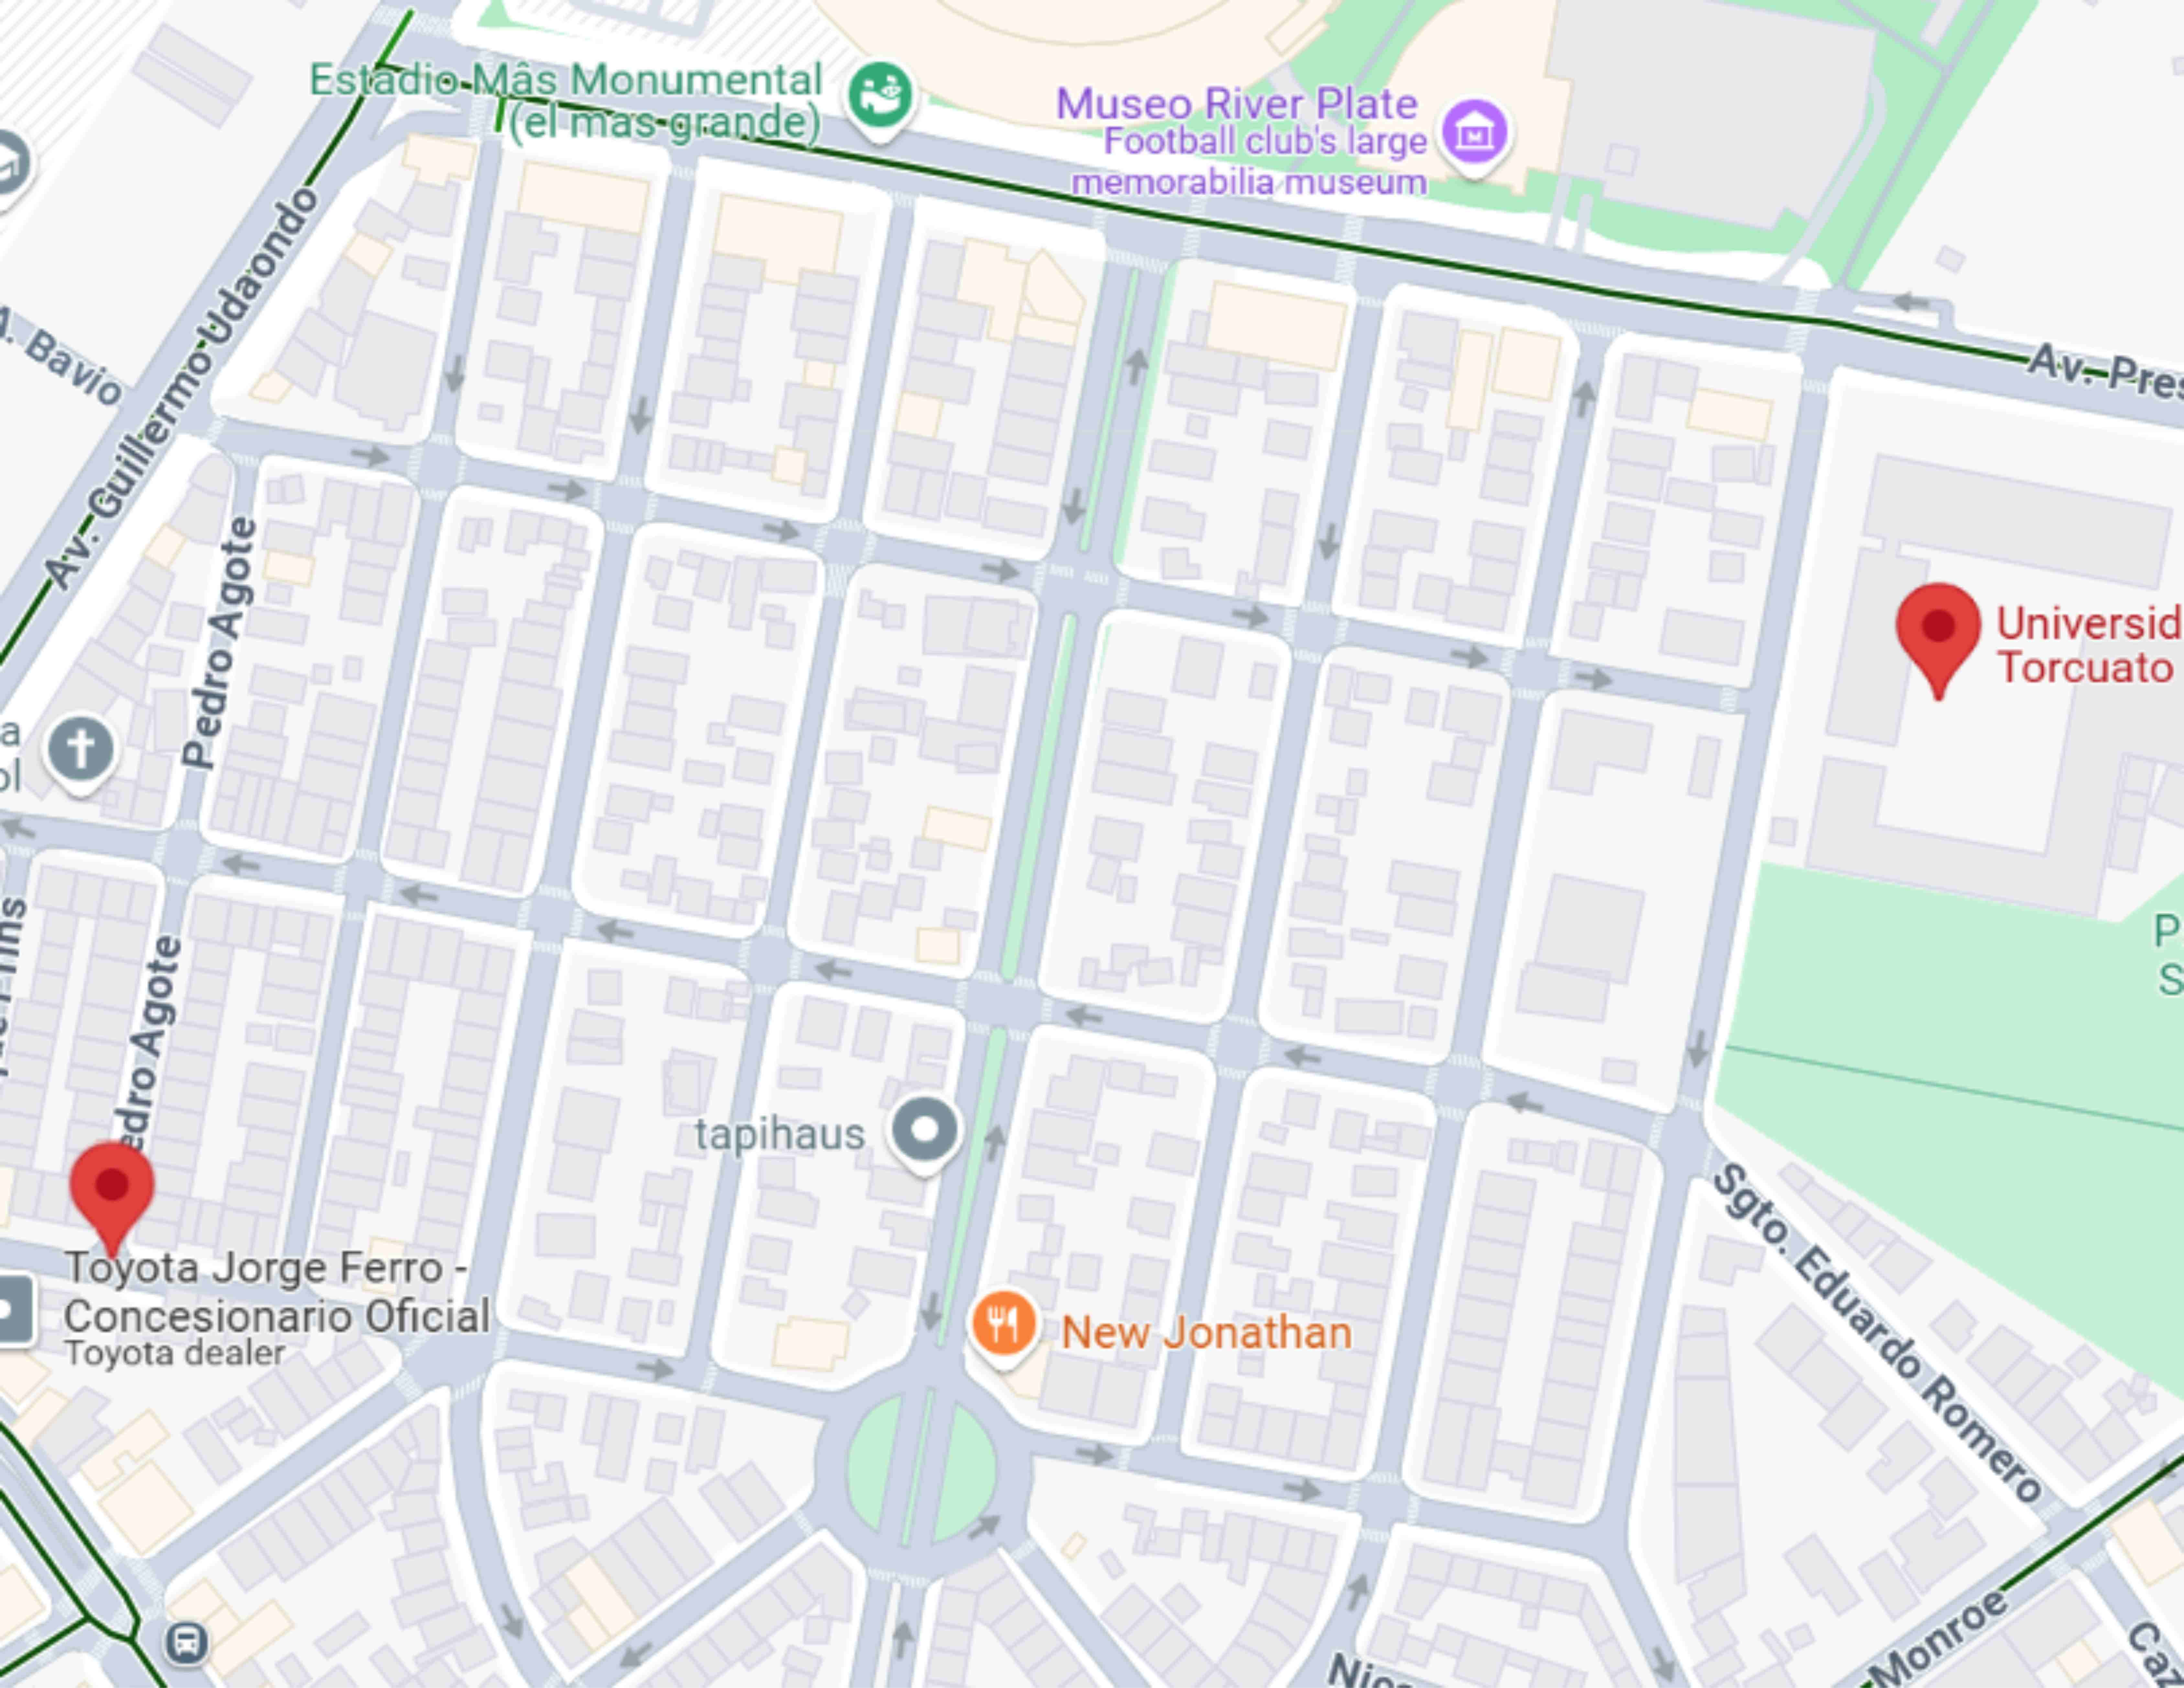
\includegraphics[width=0.9\textwidth]{../Images/Figures/mapa.jpg}
\end{center}
\end{frame}
\begin{frame}{Ejemplo: Ruta de Casa a La Universidad}
\begin{itemize}
\item Modelo MDP:
\begin{itemize}
\item<2-> Estado = posición en el mapa, en las esquinas
$x = (i,j)$
\item<3-> Acciones = desplazamiento, una cuadra por vez: 
$$
A = \left\{(0,1),(0,-1),(-1,0),(1,0)\right\} \equiv \left\{{\rm N}, {\rm S}, {\rm O}, {\rm E}\right\}
$$
\item<4-> Transición (determinística):
$$
x_{t+1} = \begin{cases}
x+a & {\rm if~}x_t \neq x^* \\
x^* & {\rm if~}x_t = x^*
\end{cases}
$$
\item<5-> Recompensa (castigo, en este caso):
$$
r_a(x) = 
\begin{cases} {\rm E}_w\left[tiempo(x,x+a,w)\right] & {\rm if}~ x \neq x^*\\
0 & {\rm if}~ x = x^*
\end{cases}
$$
\item<6-> Criterio de optimalidad:
$$
\min_u {\rm E}\left[\sum\limits_{t=0}^\infty r_u(x_t)\right].
$$
\end{itemize}
\item<7-> Implementación en Python de iteración de valor e iteración de políticas
\end{itemize}
\end{frame}

\begin{frame}{Interpretación}
\begin{itemize}
\item Diagrama para iteración de política
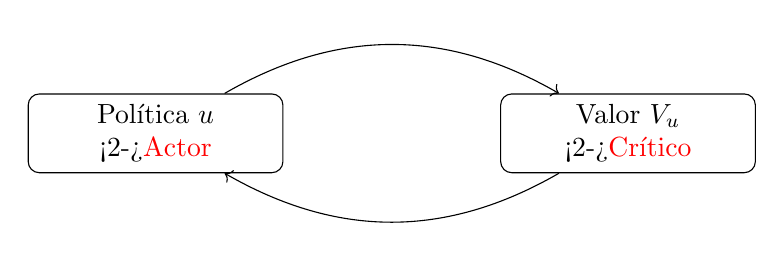
\begin{tikzpicture}[node distance=6cm]
  \node (politica) [startstop] {Política $u$ \\ \only<2->{\textcolor{red}{Actor}}};
  \node (valor) [startstop, right of=politica] {Valor $V_{u}$ \\ \only<2->{\textcolor{red} {Crítico}}};
 \draw [->, bend left=30] (politica) to (valor);
  \draw [->, bend left=30] (valor) to (politica) ;
\end{tikzpicture} 
\item<2-> Algoritmo actor-crítico
\begin{itemize}
\item<3->{\bf Actor} selecciona una politica $u_k$ (por ejemplo, codiciosa con respecto a $V_{u_{k-1}}$;
\item<4->{\bf Crítico} evalúa la política, generando la función valor $V_{u_k}$
\end{itemize}
\item<5-> En iteracion de política, $V_{u}$ es la función valor exacta de $u$.
\item<6-> Se puede reemplazar $V_u$ con una aproximación $\tilde{V}_u$. Muchos algoritmos de RL tienen esa forma.
\item<7-> Iteración de valor puede ser interpretada como un caso límite de actor-critico:
\begin{itemize}
\item $u_k$ es la política codiciosa con respeto a $V_{k-1}$
\item la evaluación se vuelve $\tilde{V}_{u_k}(x) \equiv V_k = r_{u_k}(x)+\alpha\sum_y P_{u_k}(x,y)V_{k-1}(y)$
\end{itemize}
\end{itemize}
\end{frame}

\begin{frame}{Desafiós Para Aplicación de MDPs}
\begin{itemize}
\item MDPs representan un paradigma que permite modelar y, en principio, encontrar estratégias óptimas para una amplia gama de situaciones.
\item<2-> Pero... en la práctica hay varios desafíos.
\item<3-> Ejemplos:
\begin{itemize}
\item<4-> Precificación personalizada: en principio, un e-commerce podria ajustar precios para cada usuario individualmente
\begin{itemize}
\item<5-> Probabilidad de que el usuario acepte un determinado precio no es conocida de antemano
\end{itemize}
\item<6-> Gestión de relaciones con clientes: tomar decisiones de contacto o retención según el estado del cliente
\begin{itemize}
\item<7-> El estado emocional del cliente (satisfecho, dudoso, a punto de irse) no se puede observar directamente, solo hay observaciones indirectas
\end{itemize}
\item<8-> Gestión de inventario con múltiples productos:
\begin{itemize}
\item<9-> Tanto el espacio de estados (nivel de inventario de cada producto) y de acciones (cuánto más pedir de cada producto) crecen exponencialmente con el número de productos
\end{itemize}
\end{itemize}
\end{itemize}
\end{frame}

\begin{frame}{Desafíos Para la Aplicación de MDPs}
\begin{minipage}{1.07\textwidth}
\begin{block}{Información Parcial}
\begin{enumerate}
\item<2-> Parámetros del modelo desconocidos:
probabilidades de transición     y recompensas   
\visible<12->{\textcolor{red}{$\Rightarrow$ aprendizaje}}
\item<3-> Estado $x$ no siempre puede ser observado. 
\begin{itemize}
\item<4-> observaciones $h(x,w)$ con ruído $w$ 
\item<5-> POMDP: proceso markoviano de decisión parcialmente observable
\end{itemize}
\visible<14->{\textcolor{red}{$\Rightarrow$ en principio, se convierte en MDP; en la práctica, muy difícil}}
\end{enumerate}
\end{block}

\visible<6->{\begin{block}{Complejidad del Sistema}
\begin{enumerate}
\item[3]<7-> “Maldición de la dimensionalidad”
\begin{itemize}
\item<8-> Número de estados exponencial en el número de variables de estado
\begin{itemize}
\item<9->  Dificultades para almacenar $P$ y $r$ y calcular $V^*$
\end{itemize}
\item<10-> Número de acciones exponencial en el número de variables de acción
\begin{itemize}
\item<11-> $\max\limits_{a \in A}\left\{r_a(x)+\sum_y P_a(x,y)V^*(y)\right\}$
\end{itemize}
\end{itemize}

\visible<13->{\textcolor{red}{$\Rightarrow$ generalización}}
\end{enumerate}
\end{block}}
\end{minipage}
\end{frame}

\begin{frame}{Desafío: Incertidumbre Sobre Parámetros del Modelo}
\begin{itemize}
\item La metodología está basada en información que no siempre tenemos, en especial las probabilidades de transición $P$ y recompensas $r$.
\item Qué hacer? 
\item<2-> "Aprender" a partir de interacciones con el ambiente.
\item<3-> Con qué datos?
    \begin{itemize}
        \item<7-> trayectorias
        \begin{itemize}
            \item<7-> solo una: $(x_0,a_0,r_0,x_1,a_1,r_1,\dots,x_N)$ ($N$ puede ser infinito)
            \item<8-> multiples: $(x_0^i,a_0^i,r_0^i,x_1^i,a_1^i,r_1^i,\dots,x_N^i),~i=1,\dots,M$
        \end{itemize}
        \item<9-> tuplas $(x^i,a^i,r^i,y^i),~i=1,2,\dots,N$ 
    \end{itemize}
\end{itemize}

\vspace{-0.2cm}
\begin{center}
\mode<beamer>{
\only<2,3>{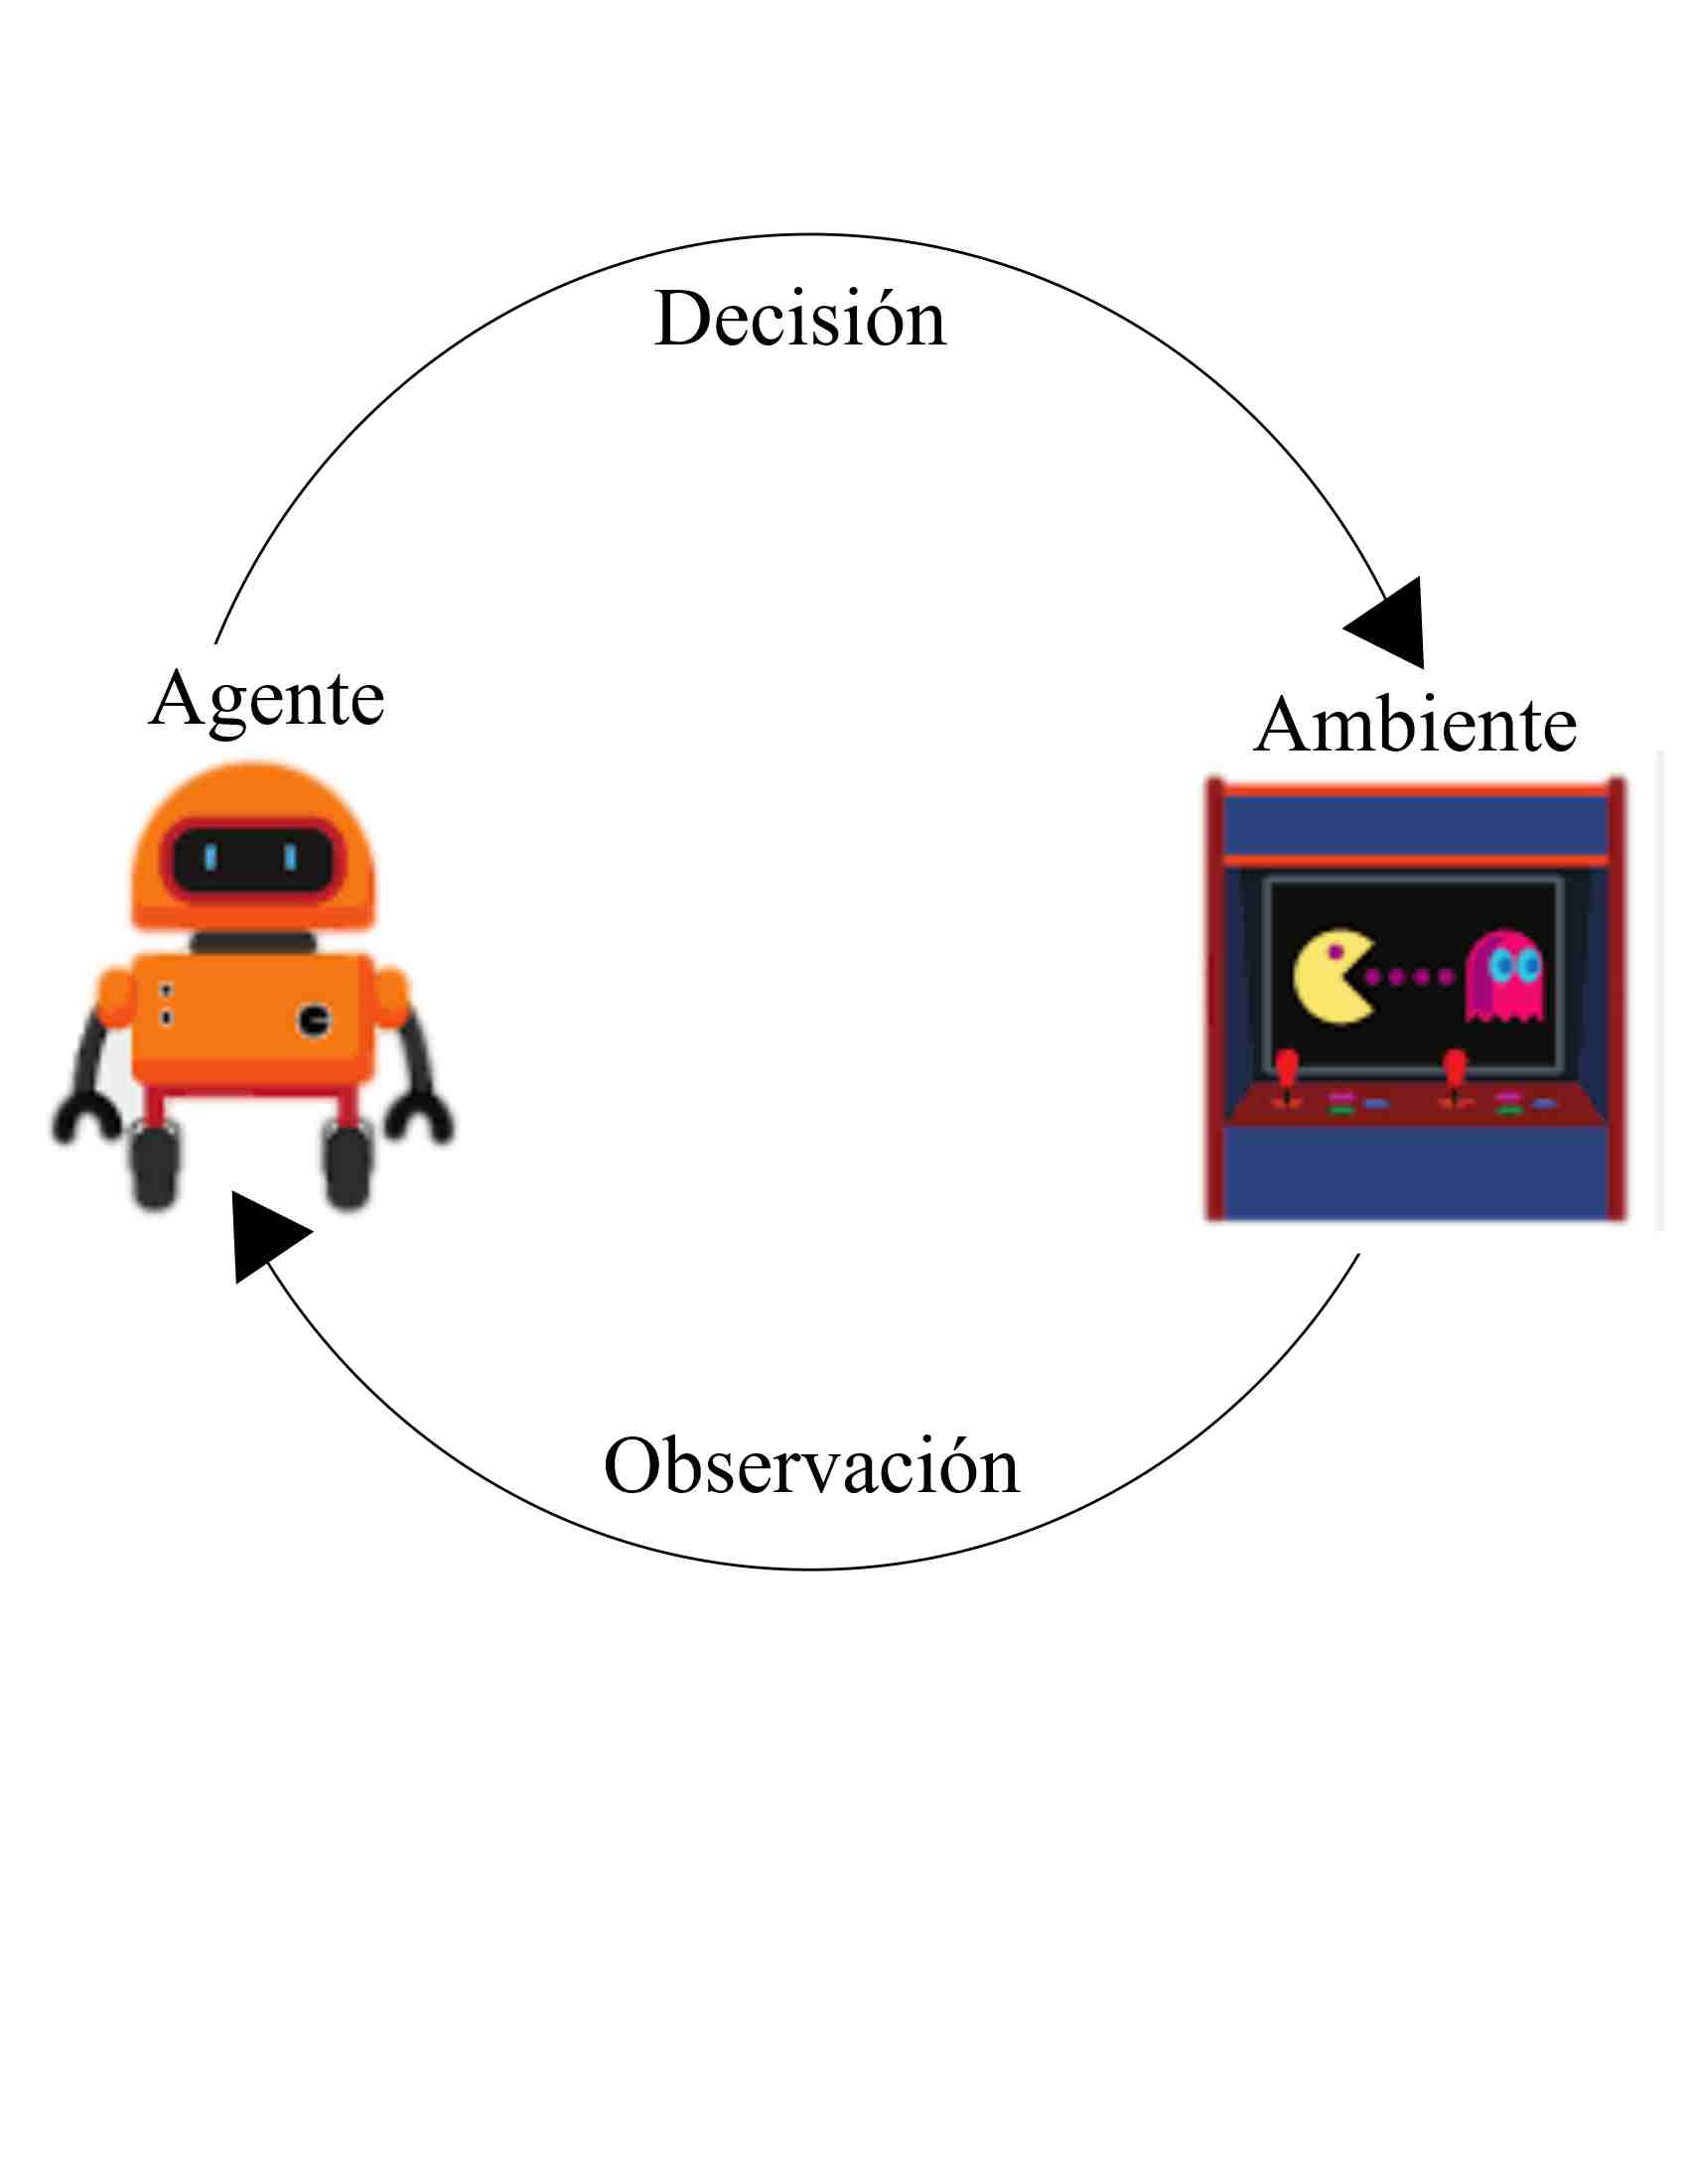
\includegraphics[width=0.35\textwidth]{../Images/LearningCycle/RL2.jpg}} 
\only<4>{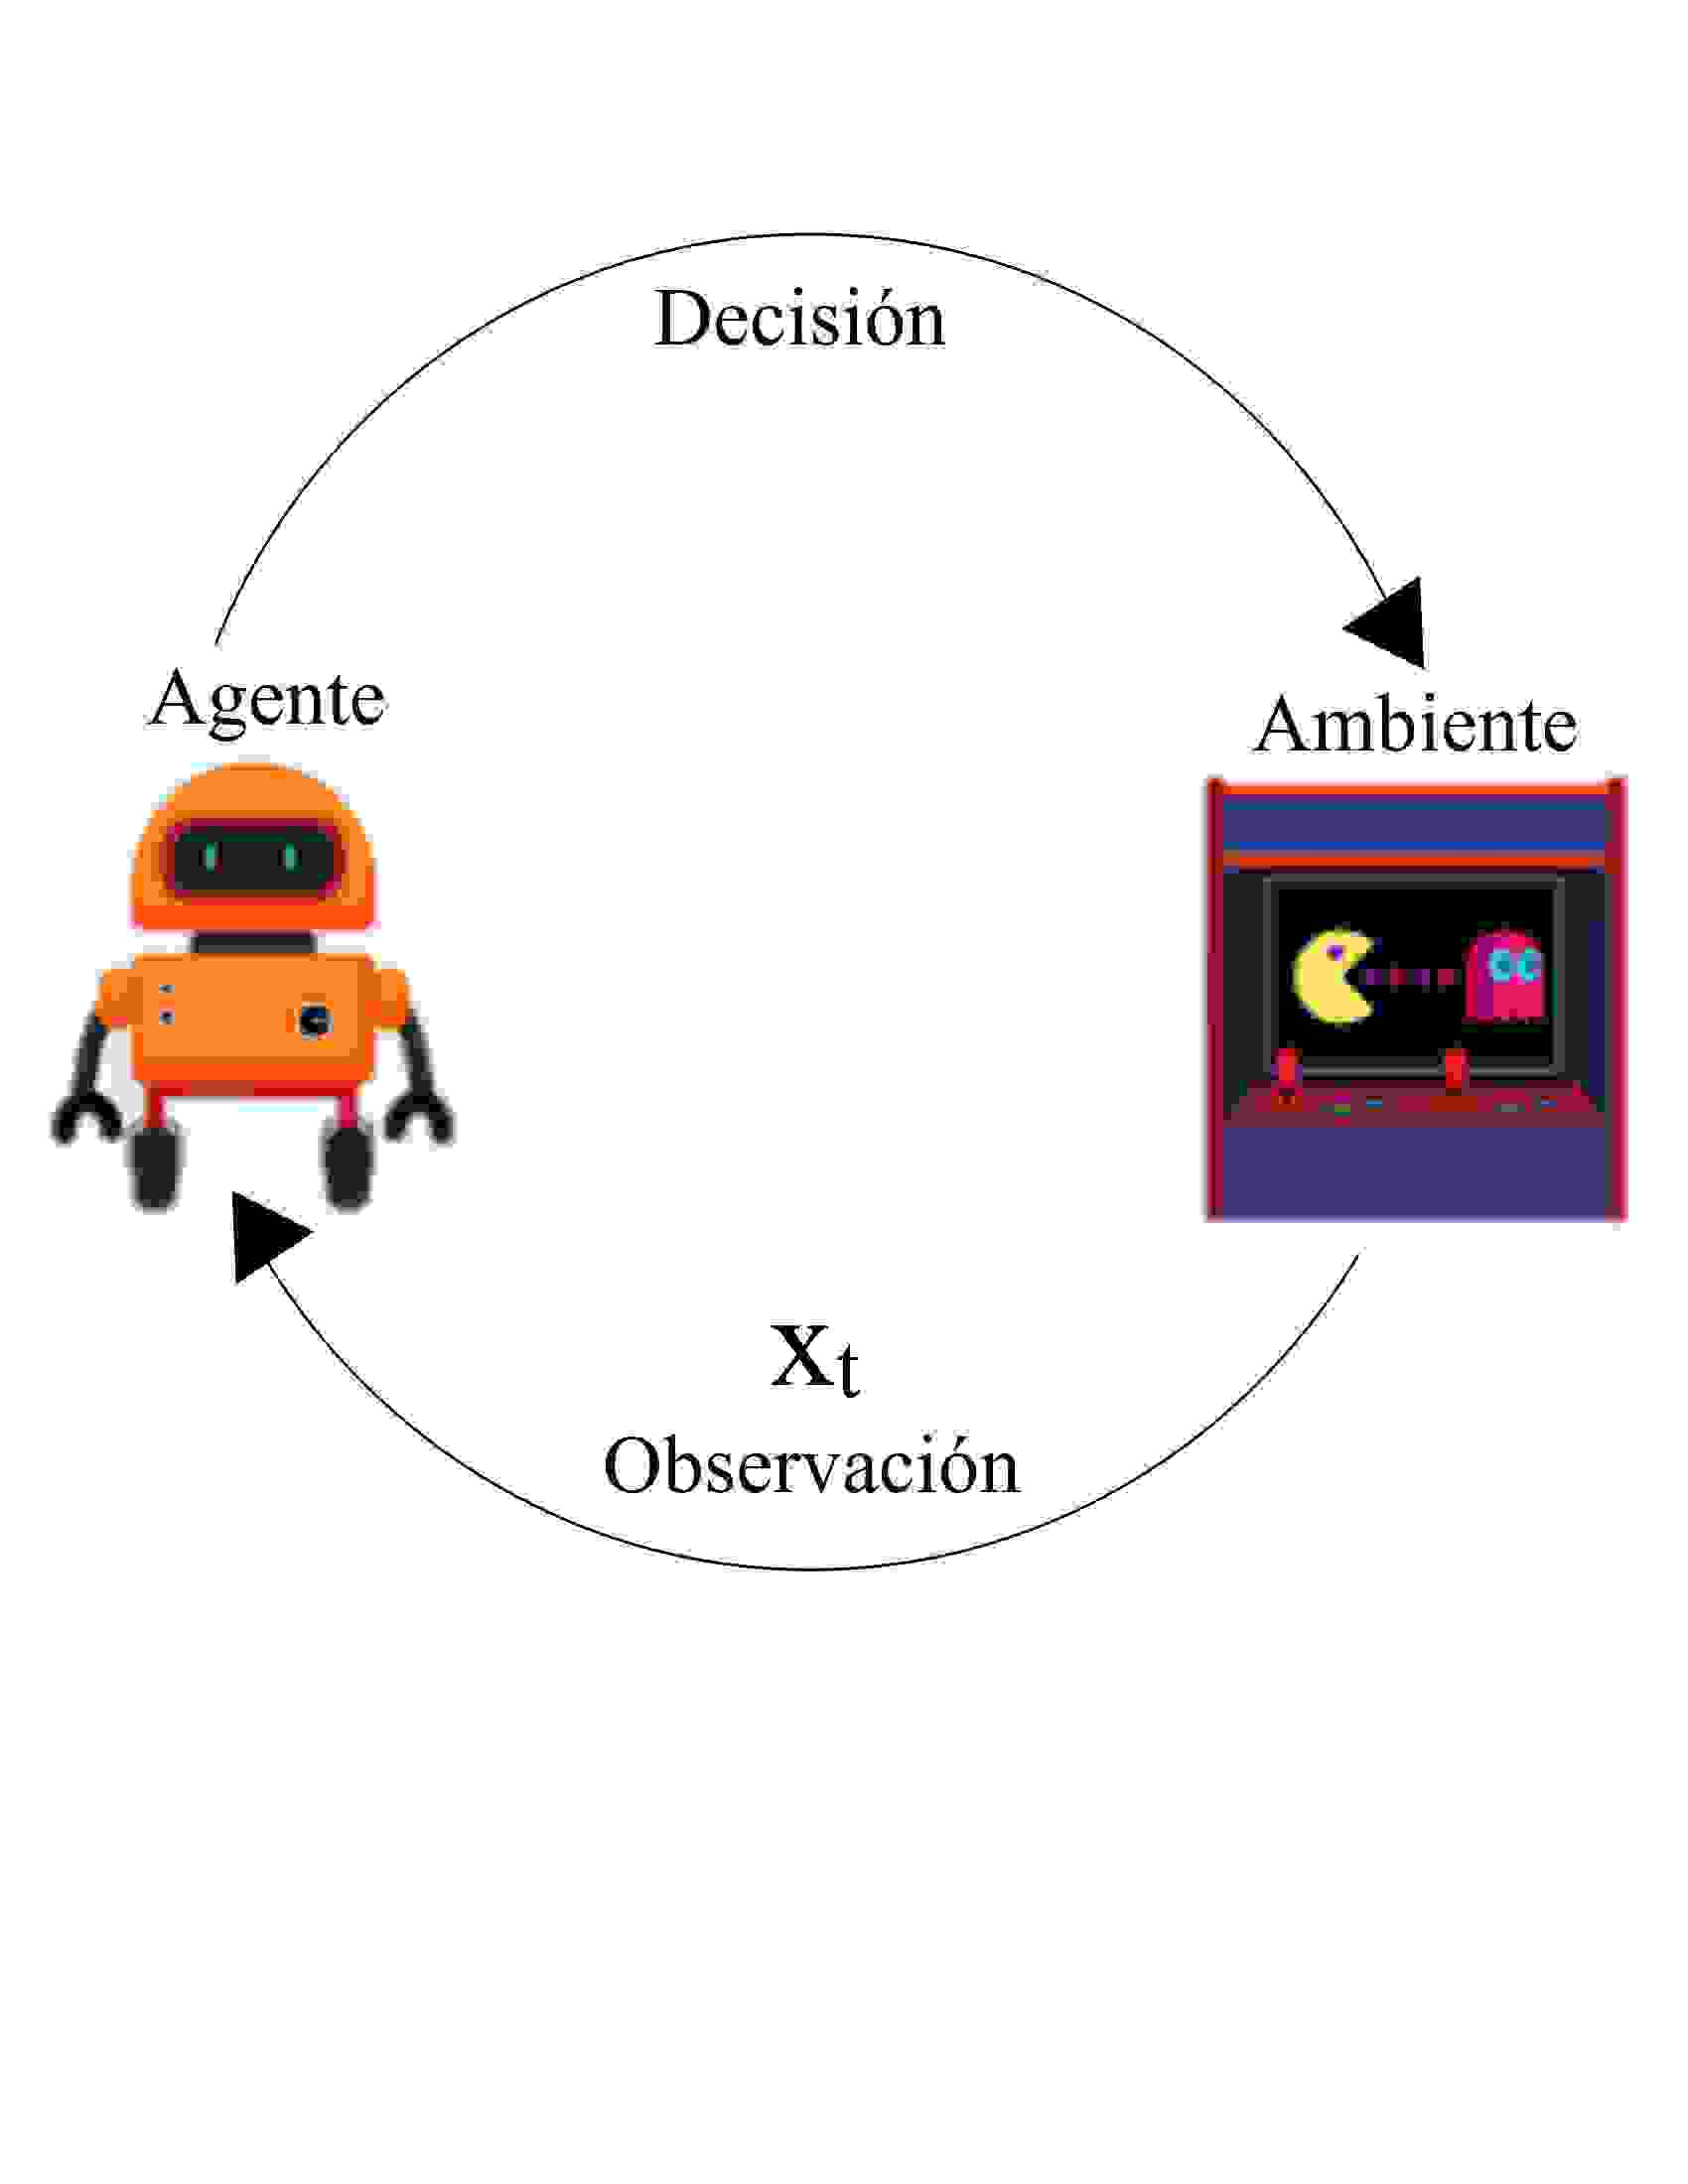
\includegraphics[width=0.35\textwidth]{../Images/LearningCycle/LearningCycle1.jpg}}  
\only<5>{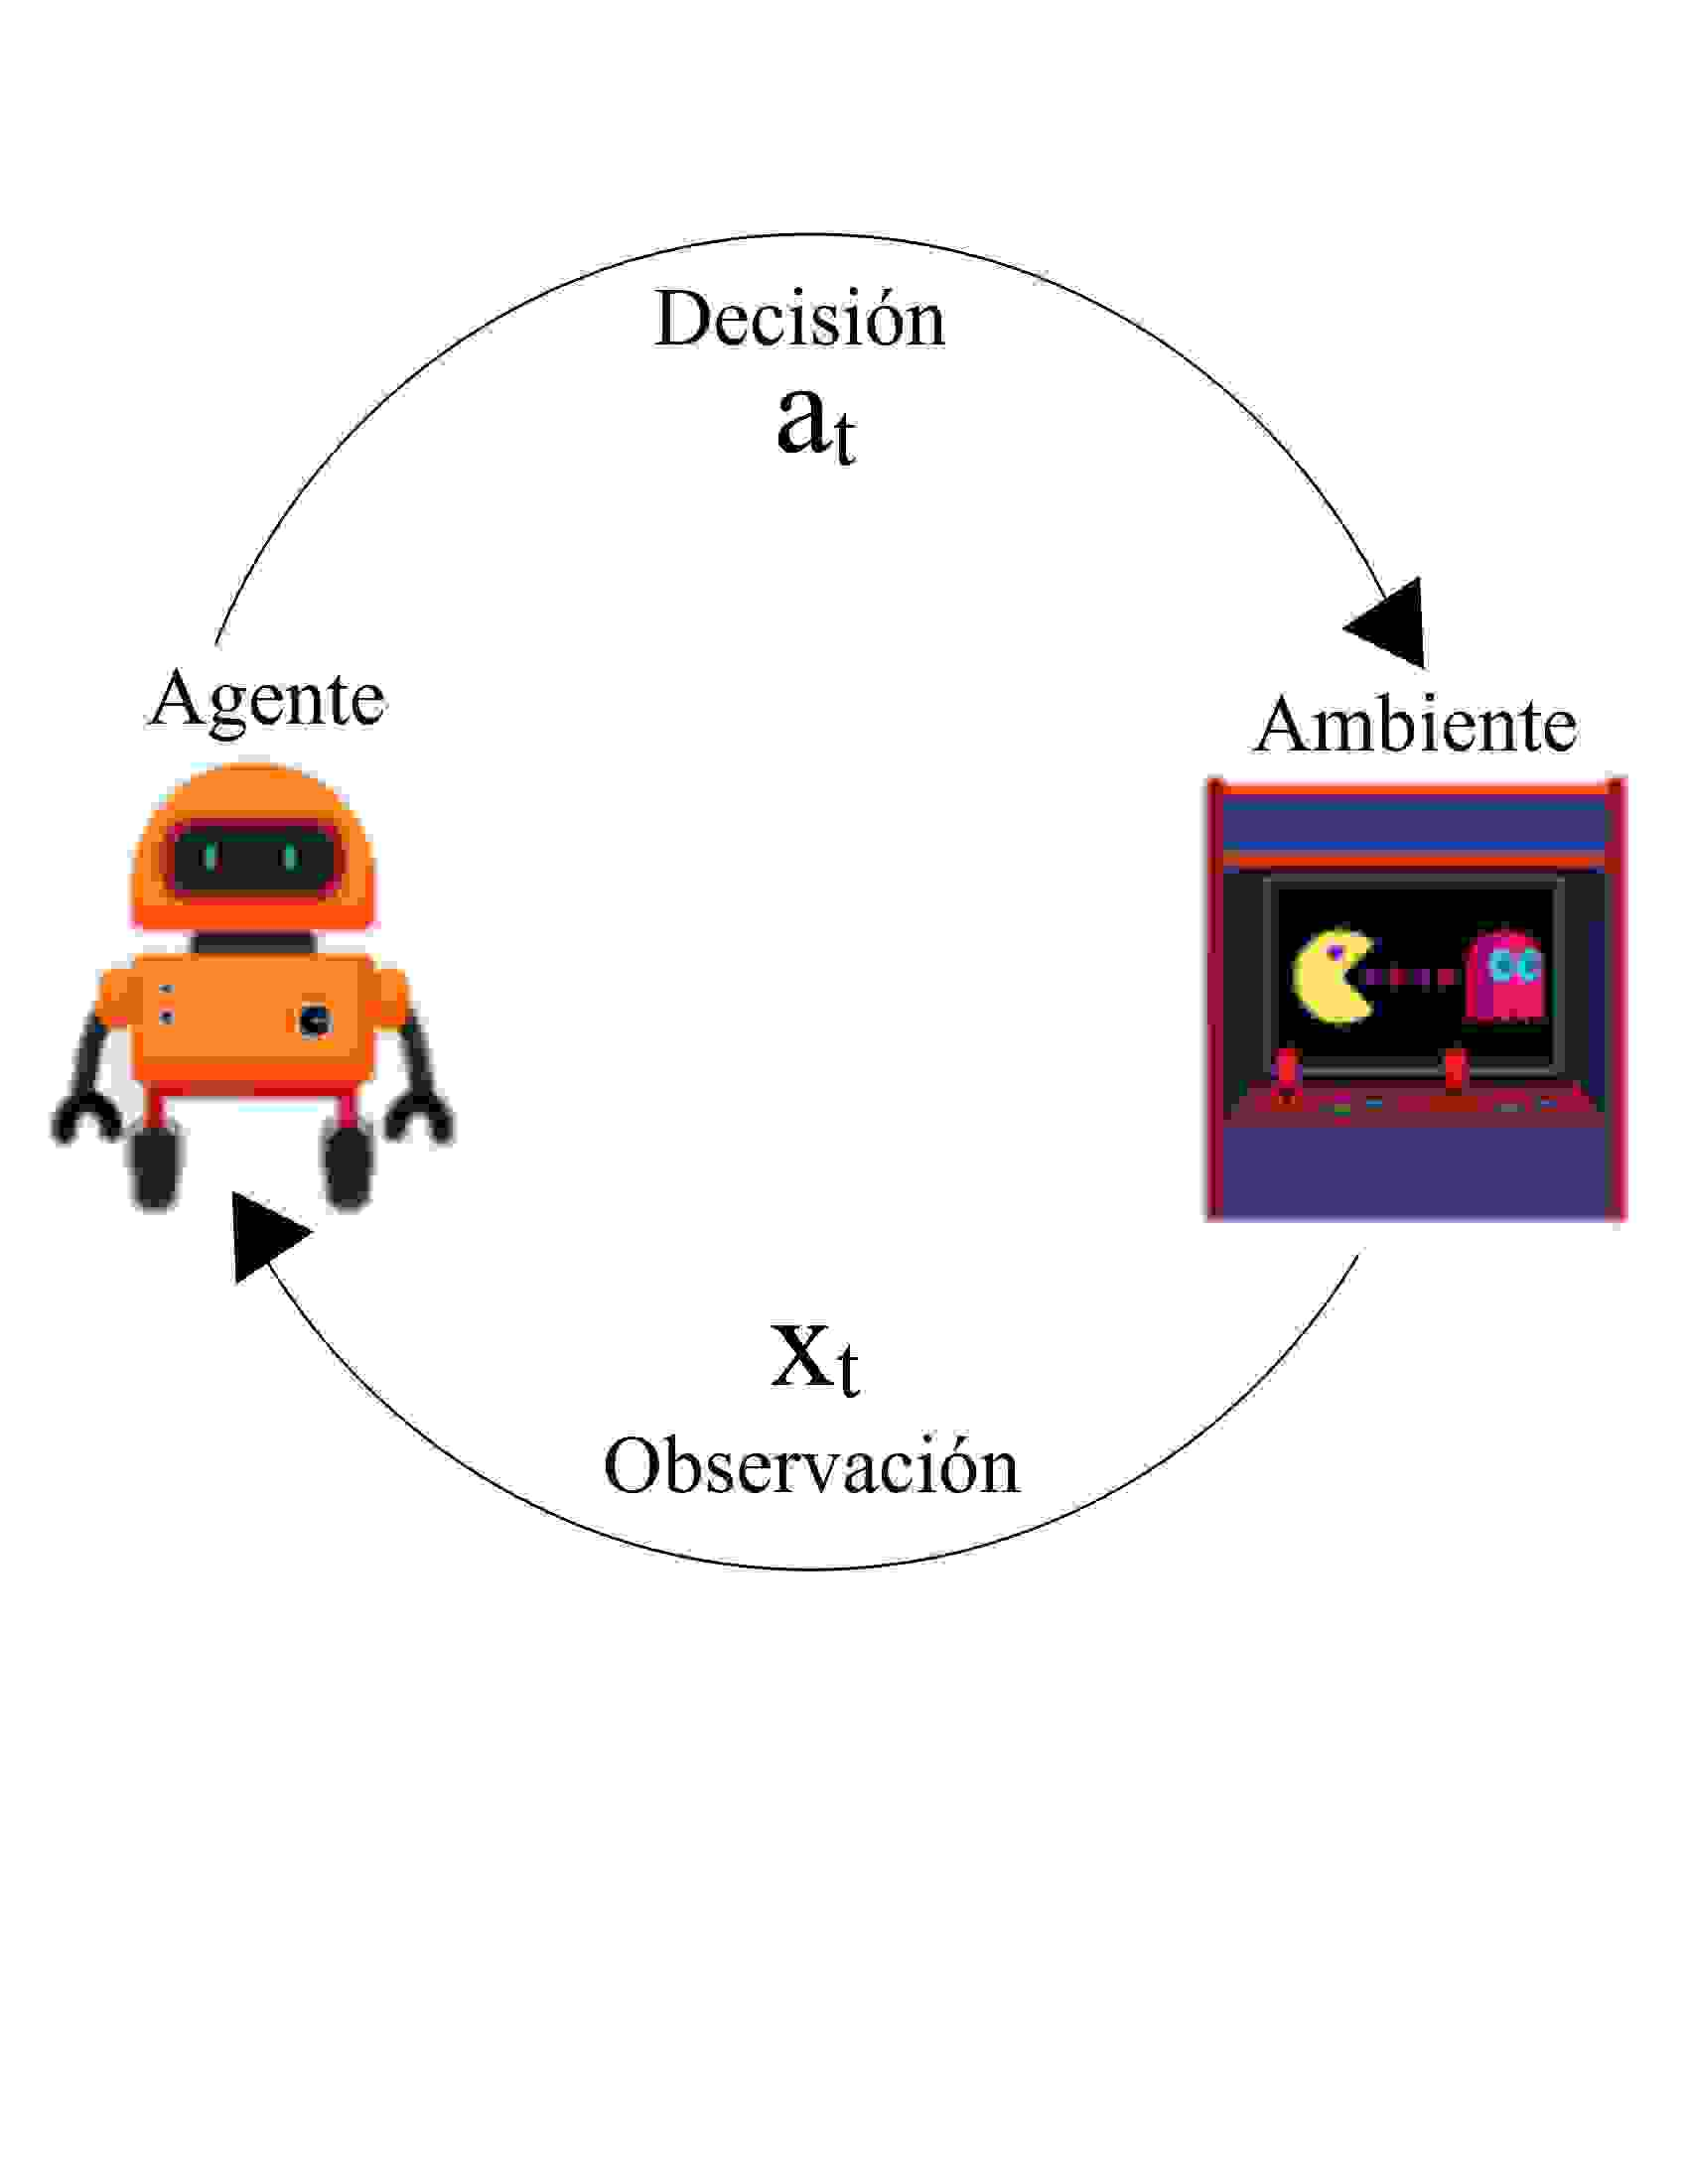
\includegraphics[width=0.35\textwidth]{../Images/LearningCycle/LearningCycle2.jpg}} 
\only<6->{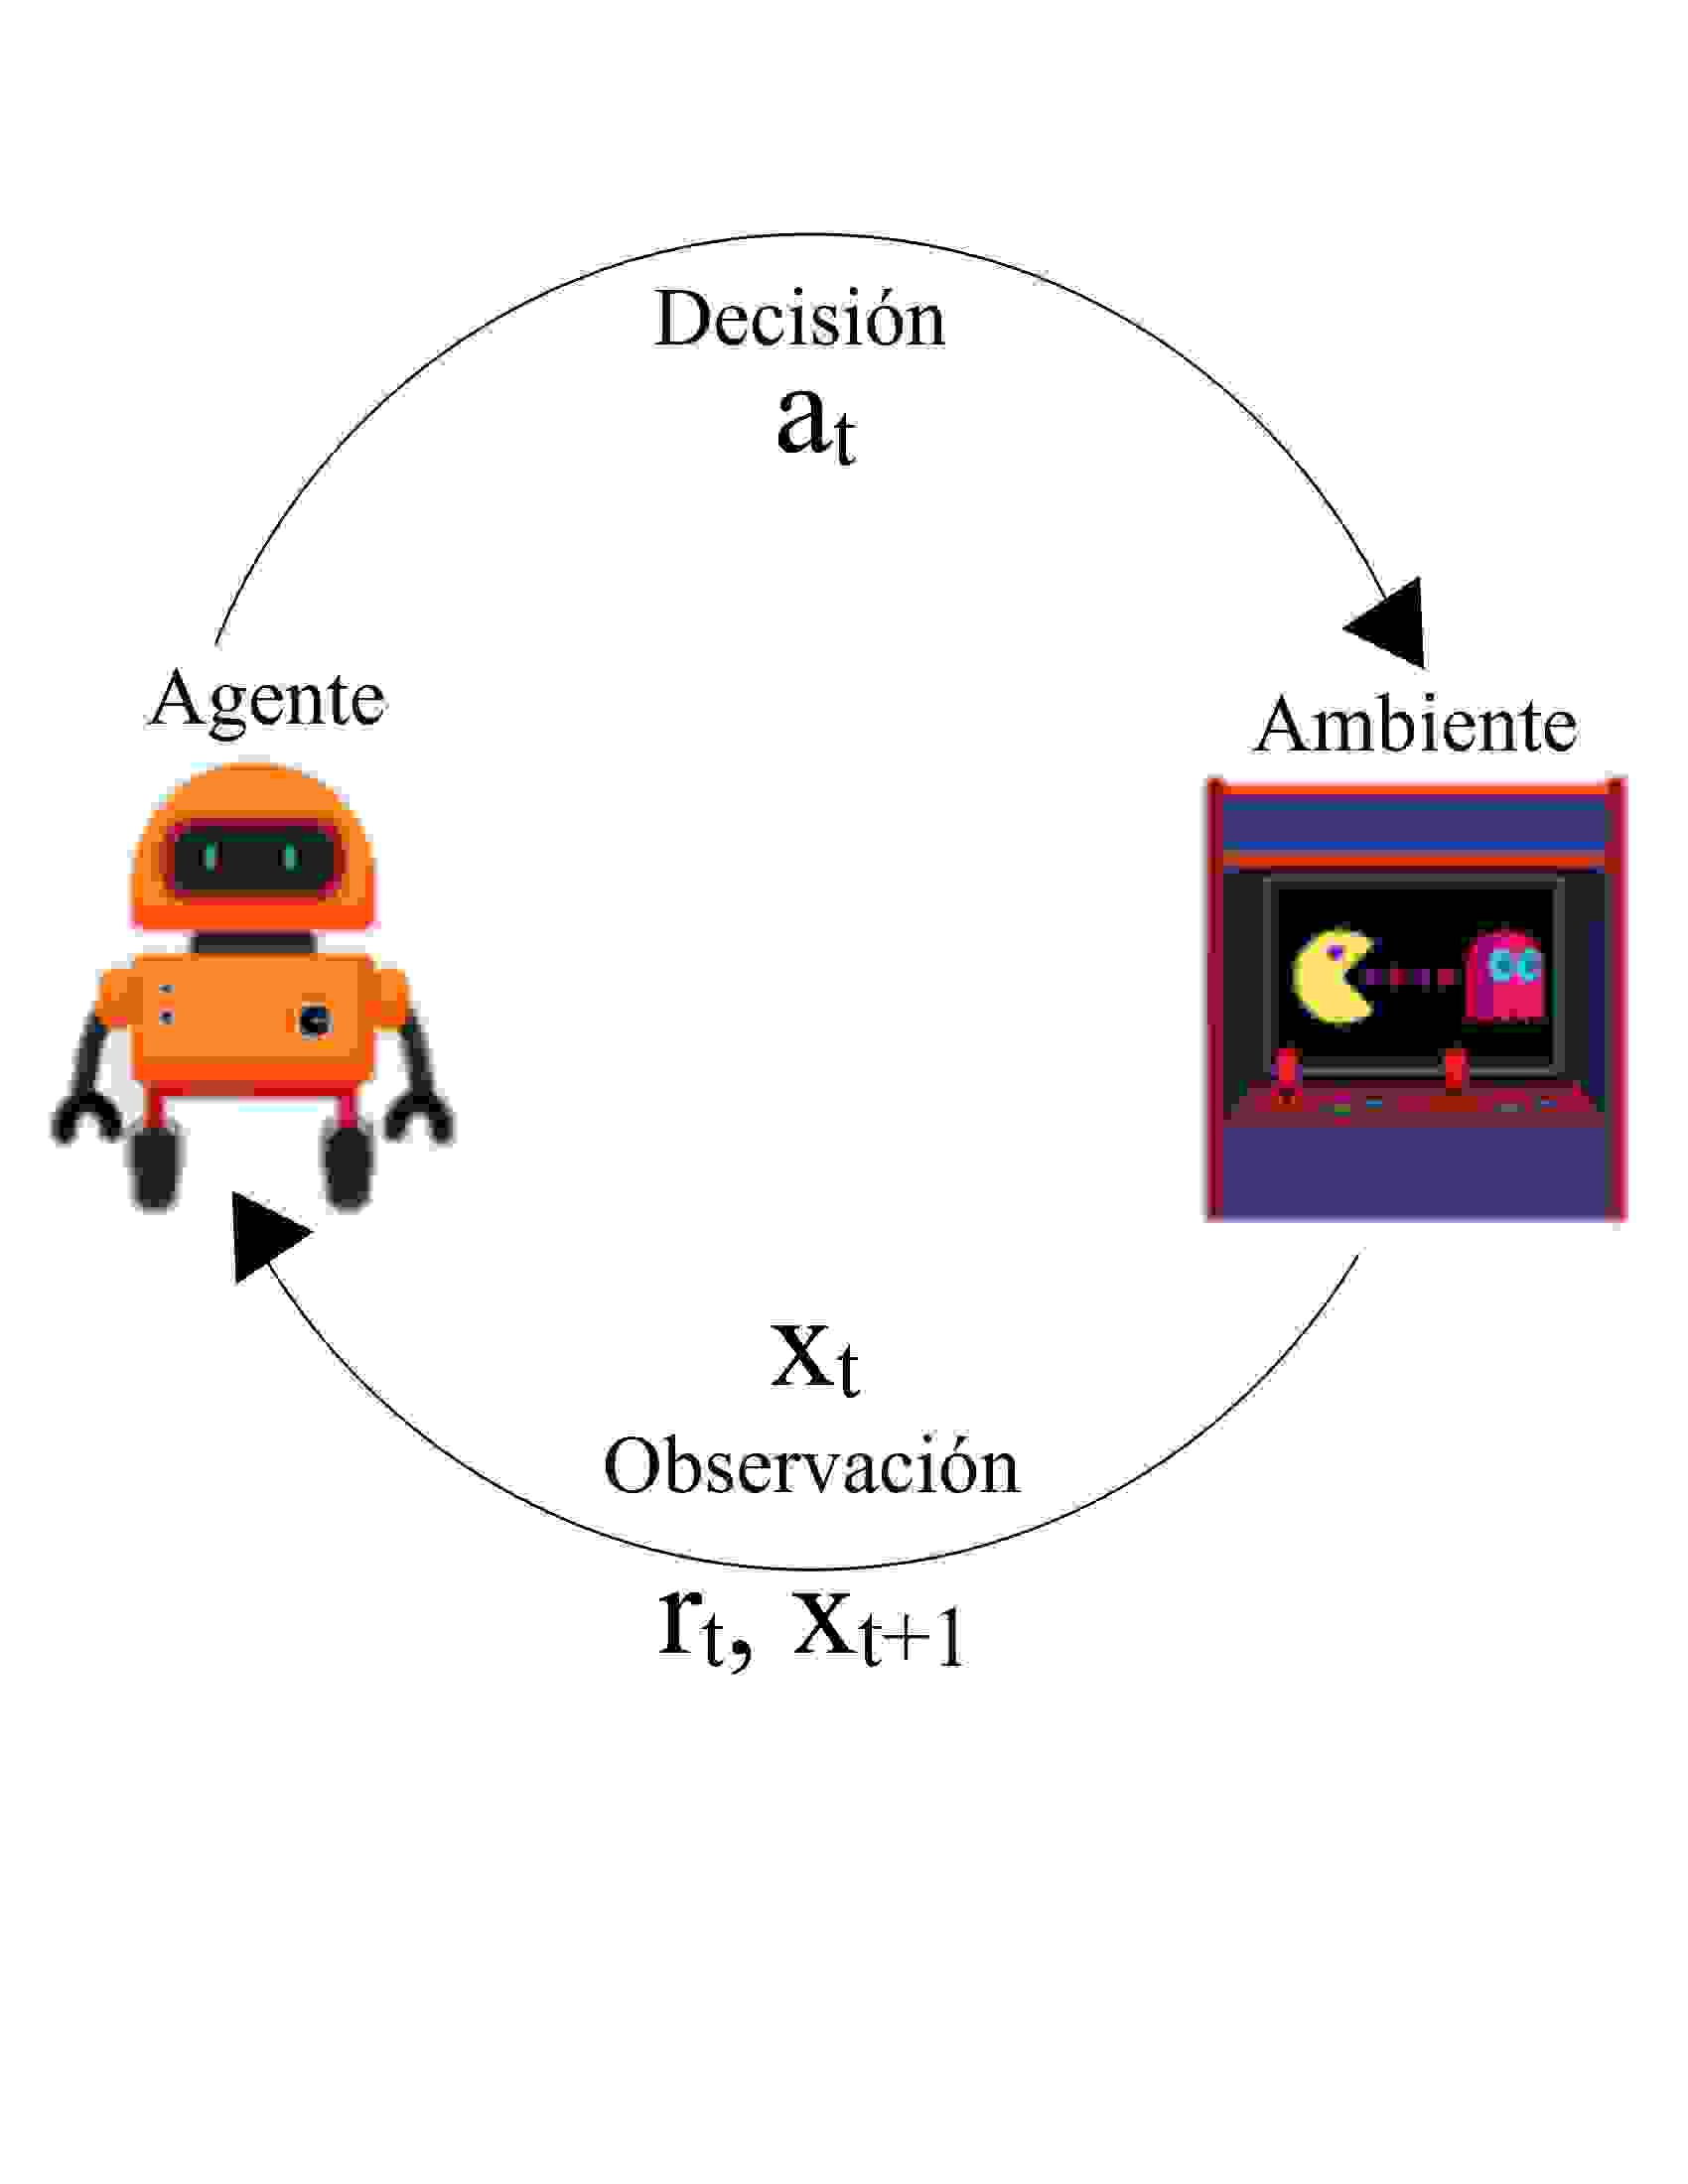
\includegraphics[width=0.35\textwidth]{../Images/LearningCycle/LearningCycle3.jpg}}} 
\end{center}
\end{frame}

\begin{frame}{Aprendizaje Por Refuerzo}
\scalebox{0.8}{
\hspace{-1cm}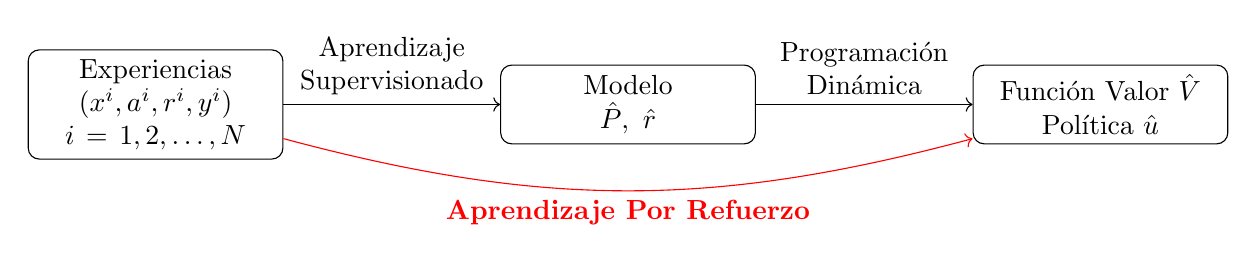
\begin{tikzpicture}[node distance=6cm]
  \node (data) [startstop] {Experiencias \\ $ (x^i,a^i,r^i,y^i)$ \\ $i=1,2,\dots,N$};
  \node<2-> (model) [startstop, right of=data] {Modelo \\ $\hat P,~\hat r$};
  \node<6-> (V_and_u) [startstop, right of=model] {Función Valor $\hat V$ \\ Política $\hat u$};
 \draw<3-> [->] (data) -- node[midway, above, align=center]{Aprendizaje \\ Supervisionado} (model);
  \draw<6-> [->] (model) -- node[midway, above, align=center]{Programación \\ Dinámica} (V_and_u);
 \draw<7-> [->, draw=red] (data) to[bend right=15] node[pos=0.5, below, align=center]{\textbf{\textcolor{red}{Aprendizaje Por Refuerzo}}} (V_and_u);
\end{tikzpicture}}
\begin{itemize}
\item Cómo ir de los datos $(x^i,a^i,r^i,y^i),~i=\dots,N$ a una política de decisión $\hat u$?
\item<2-> \textbf{Aprendiendo un modelo}
\begin{enumerate}
\item<3-> Aprendizaje supervisionado.
\begin{itemize}
\item<4-> Con $I_x = \left\{i: x^i = x\right\}$ y $I_{xy} =\left\{i:x^i=x,y^i=y\right\}$, podemos estimar:
$\hat P(x,y) = \frac{|I_{x,y}|}{|I_x|}$, $\hat r(x) = \frac{\sum_{i: \in I_x} r_i}{|I_x|}$.
\item<5-> Alternativamente, podemos estimar parámetros del sistema que permiten calcular las transiciones y recompensas (función precio x demanda, retorno y volatilidad de un activo, etc.)
\end{itemize}
\item<6-> Programación dinámica con $\hat P$, $\hat r$ $\Rightarrow$ $\hat V$, $\hat u$
\end{enumerate}
\item<7->\textbf{ Sin modelo}
\begin{itemize}
\item Aprender $\hat V$ y/o $\hat u$ directamente de los datos 

$\Rightarrow$ \textbf{aprendizaje por refuerzo } 
\end{itemize}
\end{itemize}
\end{frame}

\begin{frame}{Aprendizaje por Refuerzo: ¿Por Qué?}
\begin{itemize}
\item<1-> \textbf{Esencial cuando no es posible construir un modelo explícito del ambiente}
\begin{itemize}
    \item<2-> Hay que aprender sobre el ambiente \textbf{mientras se actúa} en él
    \begin{itemize}
        \item<3-> Ejemplo: interacción secuencial con usuarios, robots, mercados
        \item<4-> Situación enfrentada también por humanos y animales
    \end{itemize}
    \item<5-> El comportamiento del ambiente puede ser \textbf{cambiante}
    \begin{itemize}
        \item<6-> No conviene asumir una dinámica fija
    \end{itemize}
\end{itemize}

\item<7-> \textbf{Reduce suposiciones fuertes sobre la dinámica → mayor robustez}
\begin{itemize}
    \item<8-> Aprende directamente de la experiencia, sin modelo paramétrico
\end{itemize}

\item<9-> \textbf{También útil cuando se dispone de un modelo, pero...}
\begin{itemize}
    \item<10-> El modelo es demasiado complejo para resolver analíticamente (por ejemplo, no lineal o estocástico)
    \item<11-> El sistema tiene dimensión muy alta → “maldición de la dimensionalidad”
    \item<12-> El modelo solo está disponible como un \textbf{simulador} (caja negra)
    \begin{itemize}
        \item<13-> Ejemplo: videojuegos, simuladores de procesos industriales o financieros
    \end{itemize}
\end{itemize}
\end{itemize}
\end{frame}

\begin{frame}{Aprendizaje Por Refuerzo: Cómo?}
\begin{tikzpicture}[node distance=0.5cm]
  \node (data) [startstop] {Experiencias \\ $ (x^i,a^i,r^i,y^i)$ \\ $i=1,2,\dots,N$};
  \node (V_and_u) [startstop, right of=model] {Función Valor $\hat V$ \\ Política $\hat u$};
  \draw [->] (data) -- (V_and_u);
\end{tikzpicture}
\begin{enumerate}
\item \textbf{Optimización directa de la política} 
\begin{itemize}
\item<2-> Consideramos $\hat u(x) = u(x,\psi)$ donde $\psi \in \Re^K$ son parámetros a calibrar
\begin{itemize}
\item<2-> Comprar más mercadería en cantidad $u(x,\psi) =\psi_01(x\leq \psi_1)$
\item<3-> Ofrecer pasaje de avión a precio $u(x,\psi) =\psi_0+\psi_1 t +\psi_2 x$
\item<4-> Bid para publicidad online: estado $x=(p,v)$ = estimativa actual de (probabilidad $p$ de clic, valor esperado $v$ de compras resultantes del clic), bid = $u(x,\psi) = \psi_0+\psi_1 p +\psi_2 v$
\item<5-> Estos ejemplos utilizan parametrizaciones lineales, pero podrian también ser non lineales, incluyendo redes neuronales.
\end{itemize}
\item<3-> Resolvemos $\max\limits_{\psi \in \Re^K} {\rm E}\left[\sum_{t=0}^\infty \alpha^t r_{u(x_t,\psi)}(x_t)\right] = \max\limits_{\psi \in \Re^K} f(\psi)$.
\item<4-> Utilizamos descenso estocástico de gradientes para realizar la optimización.
\end{itemize}
\end{enumerate}
\end{frame}

\begin{frame}{Aprendizaje Por Refuerzo: Cómo?}
\begin{tikzpicture}[node distance=0.5cm]
  \node (data) [startstop] {Experiencias \\ $ (x^i,a^i,r^i,y^i)$ \\ $i=1,2,\dots,N$};
  \node (V_and_u) [startstop, right of=model] {Función Valor $\hat V$ \\ Política $\hat u$};
  \draw [->] (data) -- (V_and_u);
\end{tikzpicture}
\begin{enumerate}
\setcounter{enumi}{1}
\item \textbf{Estimación de la función valor} 
\begin{itemize}
\item<2-> Aprendizaje supervisionado/Monte Carlo 
\item<3-> Versiones de iteración de valor o iteración de políticas
\end{itemize}
\item<4-> \textbf{Métodos actor-crítico}
\begin{itemize}
\item<5-> Combinan $\hat u(x) = u(x,\psi)$ (actor) con estimación/aproximación 
de la función valor $\hat V$ (crítico) 
\item<6-> Utilizados para bajar la variancia de optimización directa de la política
\end{itemize}
\end{enumerate}
\end{frame}


\begin{frame}{Estimación de La Función Valor}
\begin{itemize}
\item La función valor es definida implícitamente por la ecuación de Bellman:
$$V^*(x) =  \max\limits_{a \in A} \left\{r_a(x)+\alpha \sum_y P_a(x,y) V^*(y)\right\}$$
\item Cómo estimarla a partir de datos?
\item<2-> Empezamos con el caso de una política fija \begin{itemize} 
\item<3-> proceso markoviano con recompensa (MRP)
\end{itemize}
\end{itemize}  
\end{frame}

\begin{frame}{Estimación de La Función Valor: Simulación Monte Carlo}
\begin{itemize}
\item Con una política fija $u$, tenemos:
$$
V(x) \equiv V_u(x) = {\rm E}\left[\sum_{t=0}^\infty \alpha^t r_u(x_t)|x_t = x\right]
$$
\item<2-> A partir de una trayectoria $(x_0,r_0,x_1,r_1,x_2,r_2,\dots)$, podemos construir muestras $(x_t,R_t),~t=0,1,\dots$ de la función $V$: 
$$
R_t = \sum_{\tau=1}^\infty \alpha^{\tau-t} r_\tau
$$
\item<3-> Para cada estado $x$ visitado en la trayectoria, definimos $T_x = \left\{t: x_t = x\right\}$ y tenemos:
$$
{\bf \hat V(x) = \frac{\sum_{t\in T_x} R_t}{|T_x|}}
$$
\end{itemize}
\end{frame}

%\begin{frame}{Simulación Monte Carlo: Versión %Iterativa}
%\begin{itemize}
%\item Para cada estado $x$, con $T_x = \left\{t: %x_t=x\right\} \equiv \left\{t_0,t_1,\dots,t_{N_x-%1}\right\}$, debemos calcular:
%$$ 
%\begin{array}{ccl}
%\hat V(x) & = & \frac{\sum_{t\in T_x} R_t}{N_x} \\
%\visible<2->{& = & \frac{N_x-1}%{N_x}\underbrace{\frac{\sum\limits_{t=t_0}^{t_{N_x-1}} R_t}{N_x-1}}_{{\rm estimativa~anterior}} + \frac{1}{N_x}\underbrace{R_{t_t}}_{{\rm nueva~muestra}}}
%\end{array}
%$$
%\item<3-> Podemos calcular estimativas iterativamente. Para cada nuevo periodo $t$, hacemos 
%$$
%\begin{array}{ccl}
%\hat V^t(x) & = & \hat V^{t-1}(x),~\forall x \neq x_t,\\
%\hat V^t(x_t) & = & (1-\gamma_t)\hat V^{t-1}(x_t) + \gamma_t R_t 
%\end{array}
%$$
%\item<4-> $0<\gamma_t<1$ se denomina %\textbf{tasa de aprendizaje} y debe satisfacer a ciertas condiciones.
%\end{itemize}
%\end{frame}

\begin{frame}{Bootstrapping}
\begin{itemize}
\item Monte-Carlo se basa en muestras $(x_t,R_t),~t=0,1,\dots$ de la función $V$, donde 
$R_t = \sum_{\tau=1}^\infty \alpha^{\tau-t} r_\tau$
\begin{itemize}
\item<2-> Solo podemos calcular las muestras después de una larga trayectoria
\item<3-> Las muestras tienen variancia que normalmente crece con el tamaño de la trayectoria
\end{itemize}
\item<4-> Podemos utilizar {\bf bootstrapping} observando las muestras se relacionan con la función valor:
$$
\begin{array}{ccl}
R_t & = & \sum\limits_{\tau =  t}^\infty \alpha^{\tau-t} r_\tau \\
\only<5->{& = & r_t + \alpha \sum\limits_{\tau=t+1}^\infty \alpha^{\tau-(t+1)}r_\tau \\}
\only<6->{& \approx & r_t + \alpha \left[V(x_{t+1})+\epsilon\right]}
\end{array}
$$
\item<7-> Podemos actualizar $\hat V(x_t)$ inmediatamente al observar la transición $(x_t, a_t, r_t, x_{t+1})$:
$$
\hat V(x_t) = (1-\gamma_t)\hat V(x_t)+\gamma_t\left[r_t+\alpha \hat V(x_{t+1})\right]
$$
donde $\gamma_t$ es la {\bf tasa de aprendizaje}.
\end{itemize}
\end{frame}

\begin{frame}{TD-Learning}
\begin{block}{Algoritmo TD-Learning}
\begin{enumerate}
\item Inicializamos $\hat V$ según alguna regla y hacemos $t=1$.
\item Con observación $(x_t,r_t,x_{t+1})$, actualizar
$$
\begin{array}{ccl}
\hat V(x_t) & = & \hat V(x_t) + \gamma_t\left[ r_t +\alpha \hat V(x_{t+1})-\hat V(x_t)\right] 
\end{array}
$$
\item Hacemos $t = t+1$ y retornamos al paso 2.
\end{enumerate}  
\end{block}
\begin{itemize}
\item<2-> Observamos que ${\rm E}\left[r_t +\alpha \hat V^{t-1}(x_{t+1})\right] = r(x_t)+\alpha\sum_yP(x,y) \hat V(y)$
\begin{itemize}
\item TD-learning es una versión estocástica de iteración por valor
\end{itemize}
\item<3-> Las muestras $(x_t,r_t,x_{t+1}),~t=0,1,\dots$ no necesitan ser parte de una trayectoria!
\end{itemize}

\end{frame}

\begin{frame}{Un Obstáculo en RL}
\begin{itemize}
\item En este curso, nos vamos a enfocar en RL basado en estimativas y aproximaciones de la función valor.
\scalebox{0.8}{
\hspace{-0.8cm}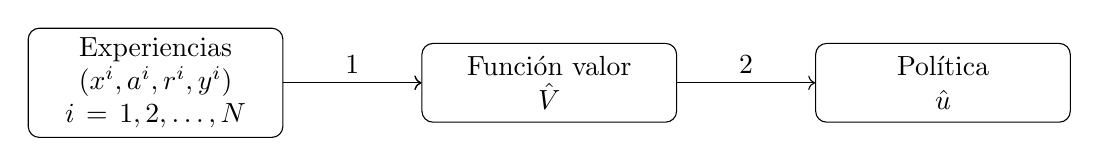
\begin{tikzpicture}[node distance=5cm]
  \node (data) [startstop] {Experiencias \\ $ (x^i,a^i,r^i,y^i)$ \\ $i=1,2,\dots,N$};
  \node (valor) [startstop, right of=data] {Función valor \\ $\hat V$};
  \node<4-> (politica) [startstop, right of=valor] {Política \\ $\hat u$};
 \draw<1,2> [->] (data) -- (valor);
\draw<3-> [->] (data) -- node[midway, above, align=center]{1} (valor);
\draw<4-> [->] (valor) -- node[midway, above, align=center]{2} (politica);
\end{tikzpicture}}
\item<2-> Conceptualmente, dos pasos:
\begin{enumerate}
\item<3-> Estimamos $V^* \approx \hat V$ a partir de $(x^i,a^i,r^i,y^i),~i=1,2,\dots$. 
\item<4-> Calculamos $\hat u$, la politica codiciosa con respeto a $\hat V$:
$$
\hat u(x) = \max_{a \in A} \left\{r_a(x) + \alpha \sum_y P_a(x,y) \hat V(y)\right\}.
$$
\end{enumerate}
\item<5-> Problema: mismo que podamos completar el paso 1), el paso 2) requiere conocimiento de $P$ y $R$.   
\item<6-> Solución basada en la \textbf{función $Q$}.
\end{itemize}
\end{frame}

\begin{frame}{La Función Q}
\begin{itemize}
\item Recordemos la ecuación de Bellman:
$$V^*(x) =  \max\limits_{a \in A} \left\{r_a(x)+\alpha \sum_y P_a(x,y) V^*(y)\right\}.$$
\item<2-> Vamos a definir 
$$Q^*(x,a) = r_a(x)+\alpha \sum_y P_a(x,y) V^*(y).$$
\item<3->  $Q^*$ satisface a otra ecuación de Bellman:
$$Q^*(x,a) = r_a(x)+\alpha \sum_y P_a(x,y) \max_{a' \in A} Q^*(y,a').$$
\item<4-> Con una aproximación $Q^* \approx \hat Q$, podemos obtener una política:
$$
\hat u(x) = \max_{a \in A} \hat Q(x,a).
$$
\item<5-> Podemos encontrar una aproximación $\hat Q$ a partir de datos utilizando TD-Learning. Con la función $Q$, ese método se denomina \textbf{Q-Learning}.
\end{itemize}    
\end{frame}

\begin{frame}{Q-Learning}
\begin{enumerate}
\item Inicializar $\hat Q$ según alguna regla y hacemos $t=1$.
\item Selectionar acción $a^i$
\item Con observación $(x^i,a^i,r^i,y^i)$, actualizar
{\small
$$
\begin{array}{ccl}
\hat Q(x^i,a^i) & = & \hat Q(x^i,a^i) + \gamma_i\left[ r^i +\alpha \max\limits_{a \in A}\hat Q(y^i,a)-\hat Q(x^i,a^i)\right] 
\end{array}
$$}
\item Hacer $t = t+1$ y retornar al paso 2.
\end{enumerate}  
\end{frame}

\begin{frame}{Q-Learning - Intuición}
\mode<beamer>{\only<1>{$$
\hat Q(x^i,a^i) = \hat Q(x^i,a^i) + \gamma_i\left[ r^i +\alpha \max\limits_{a \in A}\hat Q(y^i,a)-\hat Q(x^i,a^i)\right]
$$}}
\visible<2->{$$
\hat Q(x^i,a^i) = \hat Q(x^i,a^i) + \gamma_i\underbrace{\left[ r^i +\alpha \max\limits_{a \in A}\hat Q(y^i,a)-\hat Q(x^i,a^i)\right]}_{\rm diferencia~temporal~(TD)}
$$}
\begin{itemize}
\item<3-> La actualización es intuitiva
\begin{itemize}
\item<4-> la diferencia temporal indica si la observación del valor de la acción $a^i$ en el estado $x^i$  es mejor o peor que nuestra estimativa $Q(x_i,a_i)$
\item<5-> la estimativa es actualizada en proporción a la diferencia temporal 
\end{itemize}
\item<6-> Q-learning también es una versión estocástica de iteración de valor
\end{itemize}
\end{frame}

\begin{frame}{Q-Learning - Convergencia}
\begin{itemize}
\item Tenemos: 
$$
\hat Q(x^i,a^i) = \hat Q(x^i,a^i) + \gamma_i\left[ r^i +\alpha \max\limits_{a \in A}\hat Q(y^i,a)-\hat Q(x^i,a^i)\right]
$$
\item<2-> Definimos $I_{x,a} = \{i: (x^i,a^i) = (x,a)\}$ como el conjunto de ocurrencias de $(x,a)$ en nuestra muestra.

\item<3-> Entonces $\hat Q \rightarrow Q^*$ si:
$$
\sum_{i \in I_{x,a}} \gamma_i = \infty, ~\sum_{i \in I_{x,a}} \gamma_i^2  <\infty~~\forall (x,a).
$$
\item<4-> Observaciones:
\begin{itemize}
\item<5-> todos los pares $(x,a)$ tienen que ser visitados "infinitas veces"
\item<6-> no es necesario visitarlos en ningún orden específico
\begin{itemize}
\item<7-> convergencia a $Q^*$ asegurada sin necesidad de seguir una política específica
\end{itemize}
\end{itemize}
\end{itemize}
\end{frame}

\begin{frame}{Exploración vs. Explotación}
\begin{itemize}
\item<1-> En Q-learning, para garantizar convergencia teórica, es necesario que todos los pares $(x, a)$ sean visitados infinitas veces.
\item<2-> En la práctica, debemos equilibrar
\textbf{explotación} (usar lo que ya sabemos)  con \textbf{exploración}(probar cosas nuevas)
\item<3-> Si elegimos siempre la acción codiciosa:
$a^i = \arg\max_{a \in A} \hat Q(x^i,a)$
corremos el riesgo de ignorar acciones que podrían ser mejores
\item<4-> Solución clásica: \textbf{política \(\epsilon\)-codiciosa}
$$
a^i = \begin{cases}
\arg\max\limits_{a \in A} \hat Q^{i-1}(x^i,a) & \text{con probabilidad } 1 - \epsilon \\
\text{acción aleatoria} & \text{con probabilidad } \epsilon
\end{cases}
$$
\item<5-> En general, \(\epsilon\) puede decaer con el tiempo:
\[
\epsilon_t = \frac{1}{1 + t},\quad \text{o bien: } \epsilon_t = \epsilon_0 \cdot \beta^t
\]
\item<6->{¿Cuándo es conveniente mantener un poco de exploración incluso al final del entrenamiento?}
\end{itemize}

\end{frame}


\begin{frame}{Tasa de Aprendizaje}
$$
\hat Q(x^i,a^i) = \hat Q(x^i,a^i) + \gamma_i\left[ r^i +\alpha \max\limits_{a \in A}\hat Q(y^i,a)-\hat Q(x^i,a^i)\right]
$$
\begin{itemize}
\item<2-> \textbf{¿Qué hace la tasa de aprendizaje $\gamma_i$?}
\begin{itemize}
  \item Controla cuánto pesan las nuevas observaciones frente a lo aprendido previamente
\end{itemize}
\item<3-> Para garantizar convergencia debemos tener: $
\sum_{i \in I_{x,a}} \gamma_i = \infty, ~\sum_{i \in I_{x,a}} \gamma_i^2  <\infty~~\forall (x,a).
$
\item<4-> \textbf{Si $\gamma_i$ decae demasiado lentamente:}
\begin{itemize}
  \item Aprendizaje rápido, pero inestable
  \item Q puede oscilar mucho con recompensas ruidosas
\end{itemize}
\item<5-> \textbf{Si $\gamma_i$ decae demasiado rápido:}
\begin{itemize}
  \item Aprendizaje lento, puede estancarse
  \item Difícil adaptarse si el entorno cambia
\end{itemize}
\item<6-> $\alpha_t(x,a) = \frac{1}{1 + N_t(x,a)}$ satisface a esas condiciones. En la práctica, otras opciones pueden ser mejores.
\item<7-> ¿Cuándo sería útil mantener una tasa de aprendizaje constante en lugar de decreciente?
\end{itemize}

\end{frame}

\end{document}
